\documentclass{beamer}
\hypersetup{colorlinks=true,linkcolor=red}
\usetheme{Luebeck}
\useoutertheme[subsection=false]{smoothbars}
\useoutertheme{umbcfootline}

\usepackage{listings}
\definecolor{eclipse-red}{RGB}{127,0,65}
\definecolor{eclipse-green}{RGB}{63,127,95}
\definecolor{eclipse-blue}{RGB}{42,0,255}
\definecolor{eclipse-gray}{RGB}{100,100,100}
\lstset{language=Java,
        basicstyle=\scriptsize\ttfamily,
        keywordstyle=\color{eclipse-red},
        commentstyle=\color{eclipse-green},
        stringstyle=\color{eclipse-blue}\slshape,
        showstringspaces=false,
        escapechar=\$,
}


%--- Metadata -------------------------------------%
% Audience:      master students at computer science and engineering department
% Time budget:   30 min talk + 15 min questions + 15 min break
% Sructure:      start from general, go into details, leave 2-3 min for conclusions
% Thesis title:  Code coverage criteria and their effect on test suite qualities
% Goal:          Present our work, i.e. what we have done
\title{Code coverage criteria and their effect on test suite qualities}
\author[M.Kalkov \and D.Pamakha]
{\texorpdfstring
  {\begin{columns}
     \column{.45\linewidth}
     \centering
     Mikhail Kalkov\\
     \href{mailto:mikhail.kalkov@gmail.com}{\texttt{\small mikhail.kalkov@gmail.com}}
     \column{.45\linewidth}
     \centering
     Dzmitry Pamakha\\
     \href{mailto:dzmitry.pamakha@gmail.com}{\texttt{\small dzmitry.pamakha@gmail.com}}
   \end{columns}}
  {Mikhail Kalkov \and Dzmitry Pamakha}
}
\institute[Chalmers University of Technology]{
  Master Programme in Software Engineering and Technology\\
  Computer Science and Engineering Department\\
  Chalmers University of Technology\\
  Gothenburg, Sweden
}
\date[December 2013]{December 17, 2013}

\begin{document}

%--- Title frame ----------------------------------%
\begin{frame}[plain]
  \titlepage
\end{frame}

%--- Contents -------------------------------------%
\frame{
  \frametitle{Contents}

\tableofcontents
}


%--------------------------------------------------%
\section{Introduction}

%--------------------------------------------------%
\subsection{Motivational example}

%--- Frame ----------------------------------------%
\begin{frame}
  \frametitle{Motivational example}
\begin{columns}[T]
\begin{column}<2->{.5\textwidth}
  \centering
    Some program\\
    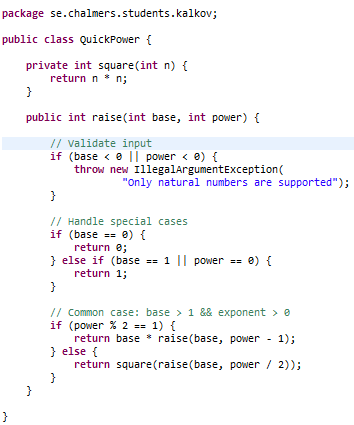
\includegraphics[scale=0.5]{QuickPower.png}
\end{column}
\begin{column}<3->{.5\textwidth}
  \centering
    Unit tests\\
    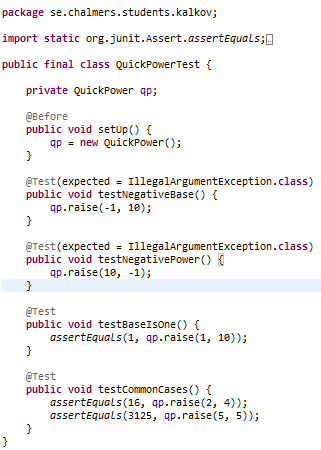
\includegraphics[scale=0.5]{QuickPowerTest.png}
\end{column}
\end{columns}
\end{frame}

%--- Frame ----------------------------------------%
\begin{frame}
  \frametitle{Motivational example}
\centering
How do you know that you have not forgotten to test some behaviour?
\end{frame}

%--- Frame ----------------------------------------%
\begin{frame}
  \frametitle{Motivational example}
\centering
It turns out many people use \emph{code coverage analysis} to answer this question.
\pause
\begin{columns}[T]
\begin{column}{.5\textwidth}
  \centering
    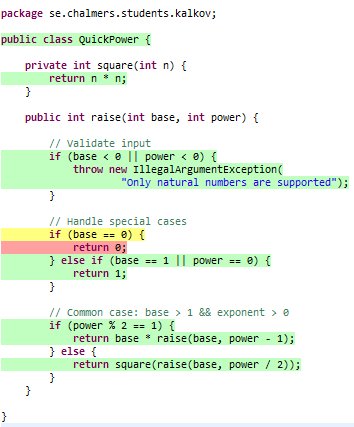
\includegraphics[scale=0.5]{QuickPower_colored.png}
\end{column}
\begin{column}{.5\textwidth}
  \centering
    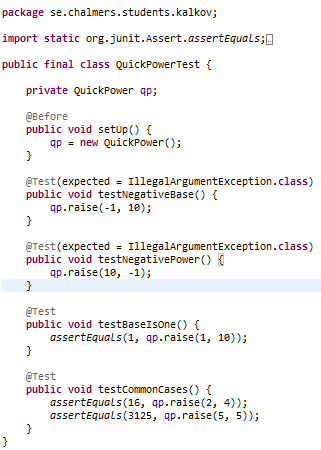
\includegraphics[scale=0.5]{QuickPowerTest.png}
\end{column}
\end{columns}
\end{frame}

%--------------------------------------------------%
\subsection{Research questions}

%--- Frame ----------------------------------------%
\begin{frame}
  \frametitle{Research questions}
\begin{itemize}
  \item What are common coverage criteria and their limits of applicability?
  \pause
  \item Which test suite qualities can be measured or affected by utilizing code coverage data?
  \pause
  \item What are common ways to present code coverage data and do they faithfully reveal
important test suite qualities?
  \pause
  \item How to implement an Eclipse plug-in for BullseyeCoverage so that code coverage data
can be fully utilized?
\end{itemize}
\end{frame}


%--------------------------------------------------%
\section{Coverage criteria}


%--------------------------------------------------%
\section{Test suite qualities}


%--------------------------------------------------%
\section{Coverage visualization}

%--- Frame ----------------------------------------%
\begin{frame}
  \frametitle{Coverage data presentation}
Case study of several code coverage tools with the following goals:
\begin{itemize}
  \item Which coverage criteria the tools support and how they present code coverage data
  \item Which test suite qualities can be measured or affected using the data from the tools
\end{itemize}
\pause
The following user stories are utilized:
\begin{itemize}
  \item Test suite completeness: reveal insufficiently tested components
  \item Test suite minimization: run only relevant test cases to decrease testing time
  \item Test suite prioritization: run tests in specific order to detect regresions quickly
  \item Test suite maintainability: easily connect test cases and parts of software under test
  \item Test case generation: generate missing test cases based on existing tests and code coverage
\end{itemize}
\end{frame}

%--- Frame ----------------------------------------%
\begin{frame}
  \frametitle{Eclemma}
Supports line, statement, method coverage for Java.
\begin{columns}[T]
\begin{column}{.7\textwidth}
    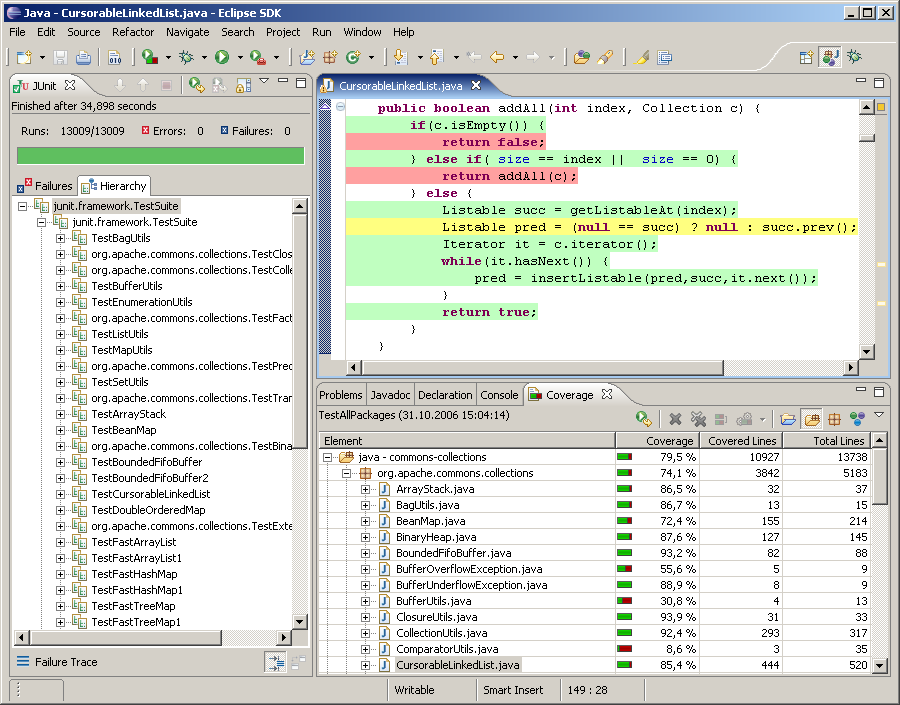
\includegraphics[scale=0.25]{eclemma.png}
\end{column}
\begin{column}{.3\textwidth}
Source code is annotated with green, red or yellow lines.\\
Coverage statistics view provides line coverage on Java sources organized as a tree.
\end{column}
\end{columns}
Eclemma addresses only the test suite completeness.
\end{frame}

%--- Frame ----------------------------------------%
\begin{frame}
  \frametitle{Clover}
Clover supports statement, decision and function criteria for Java.\newline
Like Eclemma, Clover employs source code annotations and an aggregate coverage statistics view to visualize measurements.\\
Additionally, Clover maps coverage provided by each test case to the source code.
  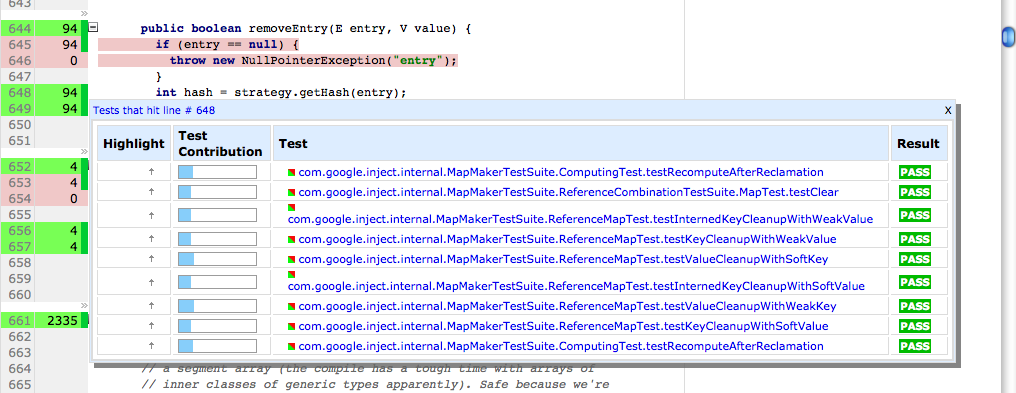
\includegraphics[width=\textwidth]{clover_mantain.png}
\end{frame}

%--- Frame ----------------------------------------%
\begin{frame}
  \frametitle{Clover}
More advaced features of Clover:
\begin{itemize}
  \item running tests based on their failure history or code changes
  \item reordering of test cases based on their comparable coverage
  \begin{item} treemap and complexity views
    \begin{columns}[T]
    \begin{column}{.5\textwidth}
         \hfill
         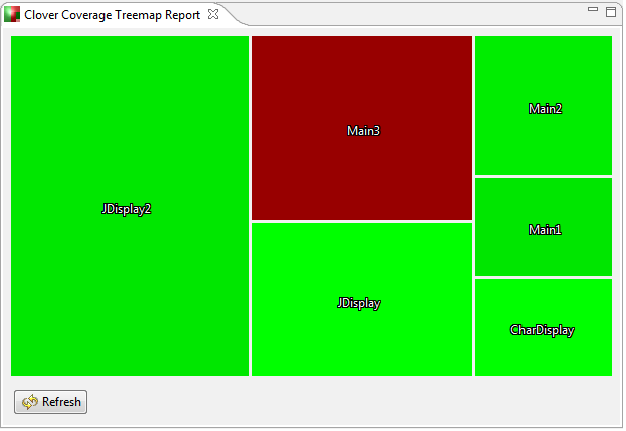
\includegraphics[scale=0.3]{clover_treemap.png}
    \end{column}
    \begin{column}{.6\textwidth}
       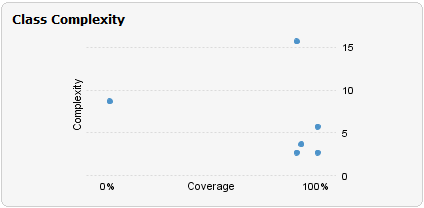
\includegraphics[scale=0.55]{clover_complexity.png}
    \end{column}
    \end{columns}
  \end{item}
\end{itemize}
Thus, Clover satisfies the test suite completeness, minimization, prioritization and maintainability stories.
\end{frame}

%--- Frame ----------------------------------------%
\begin{frame}
  \frametitle{BullseyeCoverage}
Measures coverage for C/C++ using function and condition/ decision coverage metrics by instrumenting source code after a preprocessor but before a compiler.
\begin{columns}[T]
\begin{column}{.7\textwidth}
  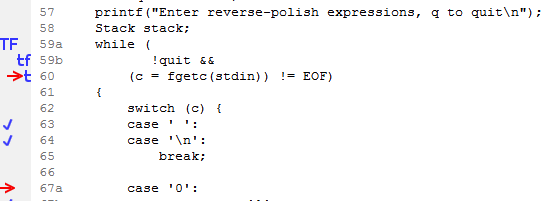
\includegraphics[scale=0.5]{bullseye_source.png}\\
  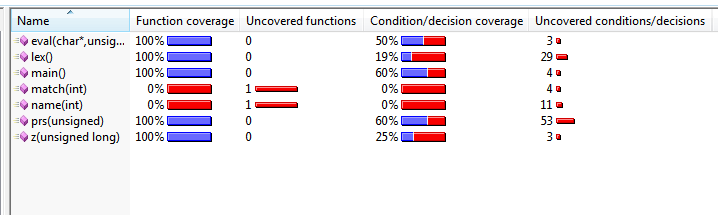
\includegraphics[scale=0.4]{bullseye_stat.png}
\end{column}
\begin{column}{.3\textwidth}
Column with coverage information is attached to read-only plain text code viewer.\\
Coverage statistics view is similar to the one used by EclEmma and Clover.
\end{column}
\end{columns}
Bullseye addresses the test suite completeness.
\end{frame}

%--- Frame ----------------------------------------%
\begin{frame}
  \frametitle{CTC++}
CTC++ is another tool for C/C++ that  supports condition/ decision coverage as well as 
more advanced multicondition coverage (MCC) and modified condition/decision coverage (MC/DC) criteria.
\begin{columns}[T]
\begin{column}{.6\textwidth}
   \hfill
    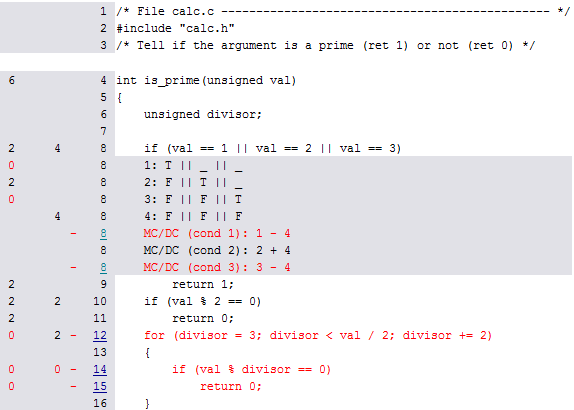
\includegraphics[scale=0.4]{ctc_source.png}
\end{column}
\begin{column}{.3\textwidth}
Coverage information is shown in HTML files in the web browser via a column attached to the source code.
\end{column}
\end{columns}
CTC++ satisfies only the test suite completeness.
\end{frame}

%--- Frame ----------------------------------------%
\begin{frame}
  \frametitle{Coverage visualization conclusion}
\begin{itemize}
  \item All examined code coverage tools support test suite completeness analysis by annotating source code with coverage information and providing a coverage summary view
  \item Other use cases are not widely supported due to lack of integration with test frameworks
\end{itemize}
Suggestions based on case analysis:
\begin{itemize}
  \item Develop code coverage tool together with a unit test framework or the whole language infrastructure 
  \item Use logarithmic “coverage ranks” scale instead of linear percentage one
  \item IDE integration helps a lot
  \item Possibility to set  boundaries of software under test
\end{itemize}
\end{frame}

%--------------------------------------------------%
\section{Bullseye plug-in for Eclipse}


%--------------------------------------------------%
\section{Conclusion}


%--------------------------------------------------%
\section{Discussion}

%--- Frame ----------------------------------------%
\begin{frame}
\begin{center}
  Thank you for attention!\\
  It is discussion time now.
\end{center}
\end{frame}

\end{document}

